\documentclass[a4paper]{article}

\usepackage{polski}
\usepackage[utf8]{inputenc}

\usepackage[export]{adjustbox}
\usepackage{scrextend}
\usepackage{amsfonts}
\usepackage{amsmath}
\usepackage{svg}

\usepackage{geometry}
\geometry{a4paper, left=15mm, top=30mm, right=15mm, bottom=20mm}

\usepackage{gensymb}
\usepackage{graphicx} 
\usepackage{isotope}
\usepackage{array}
\usepackage{float}
\usepackage{titlesec}
\usepackage{fancyhdr}
\usepackage{multirow}

\usepackage{hyperref}
\usepackage{sectsty}
\usepackage{enumitem}
\usepackage{listings}
\usepackage[labelformat=simple]{subcaption}
\usepackage{xcolor,colortbl}
\usepackage{animate}

\usepackage{karnaugh-map}

\sectionfont{\normalfont\huge\sectionrule{0pt}{0pt}{-6pt}{1pt}}
\subsectionfont{\normalfont\LARGE}
\subsubsectionfont{\normalfont\Large}

\pagestyle{fancy}
\fancyhf{}
\fancyhead[LE,LO]{\Large Łukasz Kwinta, Kacper Kozubowski, Ida Ciepiela}
\fancyhead[LE,RO]{\Large Transkoder liczb}
\fancyfoot[CE,CO]{\Large\thepage}

\renewcommand{\footrulewidth}{1pt}
\renewcommand{\headrulewidth}{1pt}

\definecolor{Gray}{gray}{0.85}
\definecolor{LightGray}{gray}{0.95}

\newcolumntype{a}{>{\columncolor{Gray}}c}
\newcolumntype{b}{>{\columncolor{white}}c}

\hypersetup{
    colorlinks,
    citecolor=black,
    filecolor=black,
    linkcolor=black,
    urlcolor=black
}

\counterwithin{table}{section}
\counterwithin{figure}{section}

\title{\fontsize{30pt}{30pt}\selectfont Laboratorium 1 \\ Transkoder liczb}
\author{\fontsize{20pt}{20pt}\selectfont Łukasz Kwinta, Kacper Kozubowski, Ida Ciepiela}
\date{marzec 2024}

\begin{document}
\maketitle
\vfill
\large
\tableofcontents

\newpage
\section{Cel zadania}
\Large Celem zadania było zaprojektować,
 zbudować i przetestować układ kombinacyjny realizujący transkoder czterobitowej liczby naturalnej (wraz z zerem)
  na sześciobitową liczbę pierwszą, bazując wyłącznie na bramkach NAND.

\section{Idea rozwiązania}
\Large Nasze rozwiązanie opiera się na przekształcaniu 4 bitów wejściowych za pomocą transkoderów, generując w rezultacie 6 bitów wyjściowych.
 Aby uzyskać konkretne kombinacje bitów wyjściowych, zastosowaliśmy funkcje logiczne opracowane z wykorzystaniem tablic Karnaugh.

\section{Układ transkodera liczb pierwszych}
\subsection{Black box}
Pierwszym krokiem w projektowaniu układu jest przedstawienie go jako tzw. "Black Box". Czyli taką czarną skrzynkę dla której 
określamy tylko wejście i oczekiwany wynik działania dla danego wejścia ale nie wgłębiamy się w implementację.

\begin{figure}[H] 
  \centering
  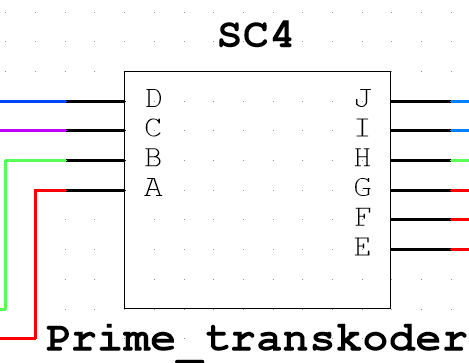
\includegraphics{black_box.png}
  \captionof{figure}{Czarna skrzynka transkodera}
\end{figure}

Wejście do układu stanowią 4 piny ABCD kodujące binarnie wejściową liczbę 0-15. Stan wysoki na pinach
stanowi logiczną jedynkę (1), a stan niski logiczne zero (0).
\begin{center}
  \begin{tabular}{|c|c|c|c|c|}
    \hline Numer bitu & 3 & 2 & 1 & 0 \\ 
    \hline Bit & A & B & C & D \\
    \hline Mnożnik & $2^3$ & $2^2$ & $2^1$ & $2^0$  \\
    \hline
  \end{tabular}
  \captionof{table}{Kodowanie pinów ABCD} 
\end{center}

Wyjście układu stanowi 6 pinów EFGHIJ kodujące pierwsze 16 liczb pierwszych. Tak samo jak na wejściu stan wysoki na pinach
stanowi logiczną jedynkę (1), a stan niski logiczne zero (0). 
\begin{center}
  \begin{tabular}{|c|c|c|c|c|c|c|}
    \hline Numer bitu & 5 & 4 & 3 & 2 & 1 & 0 \\ 
    \hline Bit & E & F & G & H & I & J \\
    \hline Mnożnik & $2^5$ & $2^4$ & $2^3$ & $2^2$ & $2^1$ & $2^0$ \\
    \hline
  \end{tabular}
  \captionof{table}{Kodowanie pinów EFGHIJ} 
\end{center}

Układ mapuje wejście na wyjście w następujący sposób - zakładając notację binarną zapisanego mapowania.

\begin{center}
  \begin{tabular}{|c|c|c|c|c|c|c|c|c|c|c|c|c|c|c|c|c|c|}
    \hline Wejście            & 0 & 1 & 2 & 3 & 4  & 5 & 6 & 7 & 8 & 9 & 10 & 11 & 12 & 13 & 14 & 15 \\ 
    \hline Oczekiwane wyjście & 2 & 3 & 5 & 7 & 11 & 13 & 17 & 19 & 23 & 29 & 31 & 37 & 41 & 43 & 47 & 53 \\ 
    \hline
  \end{tabular}
  \captionof{table}{mapowanie wejścia na wyjście} 
\end{center}

\subsection{Tabela prawdy}
Poniżej zapisaliśmy tabelę prawd dla projektowanego układu:

\begin{center}
  \begin{tabular}{|c|c|c|c||c|c|c|c|c|c|}
  \hline \multicolumn{4}{|c||}{Wejście} & \multicolumn{6}{|c|}{Wyjście} \\
  \hline A & B & C & D & E & F & G & H & I & J \\
  \hline 0 & 0 & 0 & 0 & 0 & 0 & 0 & 0 & 1 & 0 \\
  \hline 0 & 0 & 0 & 1 & 0 & 0 & 0 & 0 & 1 & 1 \\
  \hline 0 & 0 & 1 & 0 & 0 & 0 & 0 & 1 & 0 & 1 \\
  \hline 0 & 0 & 1 & 1 & 0 & 0 & 0 & 1 & 1 & 1 \\
  \hline 0 & 1 & 0 & 0 & 0 & 0 & 1 & 0 & 1 & 1 \\
  \hline 0 & 1 & 0 & 1 & 0 & 0 & 1 & 1 & 0 & 1 \\
  \hline 0 & 1 & 1 & 0 & 0 & 1 & 0 & 0 & 0 & 1 \\
  \hline 0 & 1 & 1 & 1 & 0 & 1 & 0 & 0 & 1 & 1 \\
  \hline 1 & 0 & 0 & 0 & 0 & 1 & 0 & 1 & 1 & 1 \\
  \hline 1 & 0 & 0 & 1 & 0 & 1 & 1 & 1 & 0 & 1 \\
  \hline 1 & 0 & 1 & 0 & 0 & 1 & 1 & 1 & 1 & 1 \\
  \hline 1 & 0 & 1 & 1 & 1 & 0 & 0 & 1 & 0 & 1 \\
  \hline 1 & 1 & 0 & 0 & 1 & 0 & 1 & 0 & 0 & 1 \\
  \hline 1 & 1 & 0 & 1 & 1 & 0 & 1 & 0 & 1 & 1 \\
  \hline 1 & 1 & 1 & 0 & 1 & 0 & 1 & 1 & 1 & 1 \\
  \hline 1 & 1 & 1 & 1 & 1 & 1 & 0 & 1 & 0 & 1 \\

  \hline 
  \end{tabular}
  \captionof{table}{Tabela prawdy dla układu} 
\end{center}


\subsection{Tablice Karnaugh}
Poniżej przedstawione są tabele Karnaugh których użyliśmy do zbudowania transkoderów poszczególnych bitów.
 W poniższym zapisie $A+B$ oznacza bramkę $OR(A,B)$, $AB$ oznacza $AND(A,B)$ i $\overline{A}$ oznacza $NOT(A)$.
\subsubsection{Człon J}

\begin{center}
  \begin{karnaugh-map}[4][4][1][$CD$][$AB$]
    \manualterms{0,1,1,1,1,1,1,1,1,1,1,1,1,1,1,1}
    \implicant{1}{11}
    \implicant{3}{10}
    \implicant{4}{14}
    \implicant{12}{10}
  \end{karnaugh-map}
  \captionof{table}{Tabela Karnaugh dla członu J} 
\end{center}

\begin{center}
  $f_{(1)} = \textcolor{cyan}{A}+\textcolor{green}{C}+\textcolor{red}{D}+ \textcolor{yellow}{B} $
\end{center}


\subsubsection{Człon I}

\begin{center}
  \begin{karnaugh-map}[4][4][1][$CD$][$AB$]
    \manualterms{1,1,0,1,1,0,0,1,1,0,1,0,0,1,1,0}
    \implicant{14}{10}
    \implicant{0}{1}
    \implicant{13}{13}
    \implicant{0}{4}
    \implicantedge{0}{0}{8}{8}
    \implicant{3}{7}
  \end{karnaugh-map}
  \captionof{table}{Tabela Karnaugh dla członu I} 
\end{center}

\begin{center}
  $f_{(1)} = 
    \textcolor{red}{AC\overline{D}} + 
    \textcolor{pink}{\overline{A}CD} +
    \textcolor{green}{\overline{ABC}} +
    \textcolor{cyan}{\overline{ACD}} +
    \textcolor{blue}{\overline{BCD}} +
    \textcolor{yellow}{AB\overline{C}D} $
\end{center}

\subsubsection{Człon H}
\begin{center}
  \begin{karnaugh-map}[4][4][1][$CD$][$AB$]
    \manualterms{0,0,1,1,0,1,0,0,1,1,1,1,0,0,1,1}
    \implicantedge{3}{2}{11}{10}
    \implicant{15}{10}
    \implicant{5}{5}
    \implicant{8}{10}
  \end{karnaugh-map}
  \captionof{table}{Tabela Karnaugh dla członu H} 
\end{center}


\begin{center}
  $f_{(1)} = 
    \textcolor{cyan}{A\overline{B}} + 
    \textcolor{green}{AC}+
    \textcolor{red}{\overline{B}C}+
    \textcolor{yellow}{\overline{A}B\overline{C}D} $
\end{center}

\subsubsection{Człon G}

\begin{center}
  \begin{karnaugh-map}[4][4][1][$CD$][$AB$]
    \manualterms{0,0,0,0,1,1,0,0,0,1,1,0,1,1,1,0}
    \implicant{14}{10}
    \implicant{4}{13}
    \implicant{13}{9}
  \end{karnaugh-map}
  \captionof{table}{Tabela Karnaugh dla członu G} 
\end{center}

\begin{center}
  $f_{(1)} = 
    \textcolor{green}{B\overline{C}} + 
    \textcolor{red}{AC\overline{D}}+
    \textcolor{yellow}{A\overline{C}D} $
\end{center}

\subsubsection{Człon F}

\begin{center}
  \begin{karnaugh-map}[4][4][1][$CD$][$AB$]
    \manualterms{0,0,0,0,0,0,1,1,1,1,1,0,0,0,0,1}
    \implicantedge{8}{8}{10}{10}
    \implicant{8}{9}
    \implicant{7}{6}
    \implicant{7}{15}
  \end{karnaugh-map}
  \captionof{table}{Tabela Karnaugh dla członu F} 
\end{center}

\begin{center}
  $f_{(1)} = 
    \textcolor{red}{A\overline{BD}} +
    \textcolor{green}{A\overline{BC}} +
    \textcolor{yellow}{\overline{A}BC} +
    \textcolor{cyan}{BCD} $
\end{center}

\subsubsection{Człon E}

\begin{center}
  \begin{karnaugh-map}[4][4][1][$CD$][$AB$]
    \manualterms{0,0,0,0,0,0,0,0,0,0,0,1,1,1,1,1}
    \implicant{12}{14}
    \implicant{15}{11}
  \end{karnaugh-map}
  \captionof{table}{Tabela Karnaugh dla członu E} 
\end{center}

  \begin{center}
  $f_{(1)} = \textcolor{red}{AB} + \textcolor{green}{ACD}$
\end{center}

\subsection{Implementacja}
Otrzymane z tablic Karnough funkcje zostały odpowiednio przekształcone tak,
 aby używały jedynie bramek NAND i następnie zostały one zaimplementowane. Zdecydowaliśmy się 
 na użycie schematów hierarchicznych - subcircuit - dla zwiększenia czytelnosci schematu. 
 Na pierwszym poziomie znajdują się same transkodery pojedynczych bitów - czarne skrzynki które otrzymują 
 całe wejście, a w wyniku dają konkretny bit wyjścia, innymi słowy każda funkcja logiczna została zaimplementowana
 na oddzielnym schemacie, a następnie zgromadziliśmy je w jeden podschemat stanowiący cały projektowany układ "Prime transkoder"
\begin{figure}[H]
  \centering
  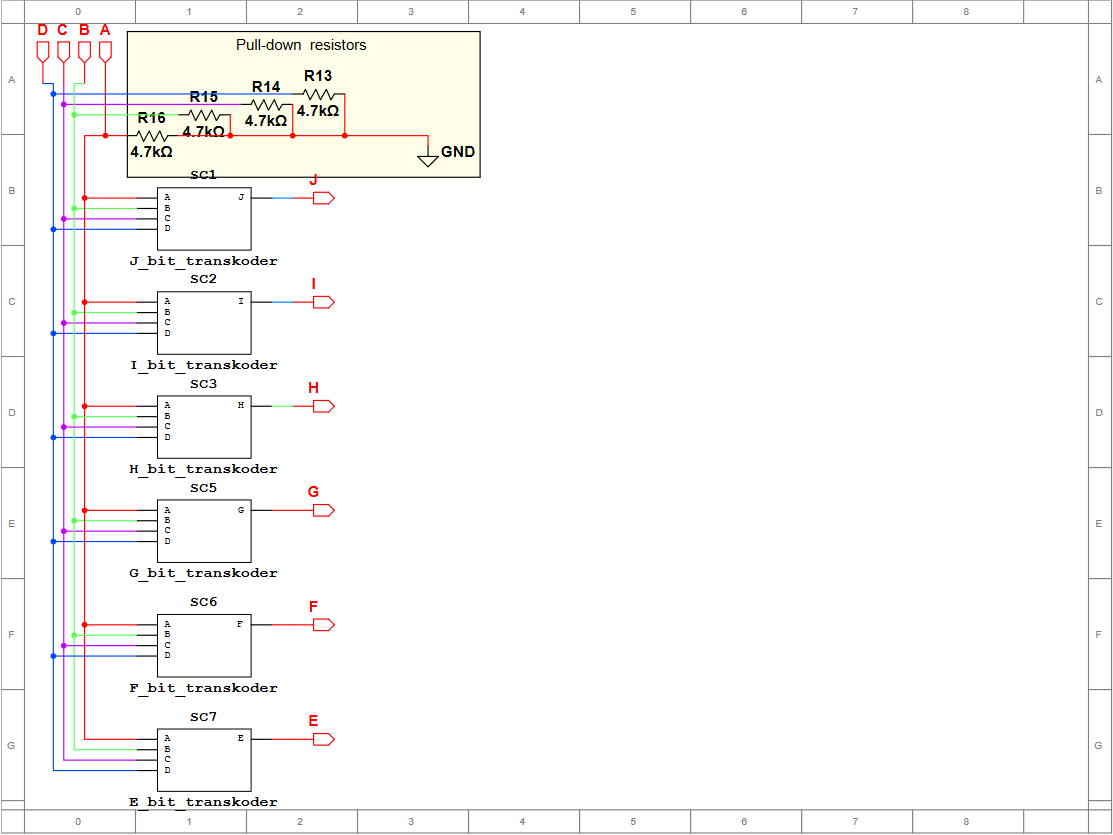
\includegraphics[width=\textwidth]{prime_transkoder.png}
  \label{Podschemat najwyższego rzędu, gromadzący w sobie podschematy właściwych funkcji logicznych}
  \captionof{figure}{Podschemat najwyższego rzędu, gromadzący w sobie podschematy właściwych funkcji logicznych} 
\end{figure}

Użyliśmy rezystorów pull-down na wejściu układu, które ściągają niepodpięty sygnał do logicznego zera aby 
zapewnić poprawne funkcjonowanie układu nawet gdy wejście nie jest podpięte w całości.

Poniżej implementacje poszczególnych funkcji logicznych zgodnie z funkcjami otrzymanymi z tablic Karnaugh razem z przekształceniami aby używane były wyłącznie bramki NAND.
Najczęściej używanymi przez nas przekształceniami będą:\\
$OR(A,B) = NAND(NOT(A),NOT(B))$\\
$AND(A,B) = NOT(NAND(A,B))$\\
$NOT(A) = NAND(A,A)$\\
Warto zauważyć, że w następującej sytuacji:\\ 
$OR(AND(A,B)) = NAND(NOT(NOT(NAND(A,B))),NOT(NOT(NAND(A,B))))$\\
Co można uprościć do poniższej formuły:\\
$NAND(NAND(A,B),NAND(A,B))$


\subsubsection{Transkoder J}
 \begin{figure}[H]
  \centering
  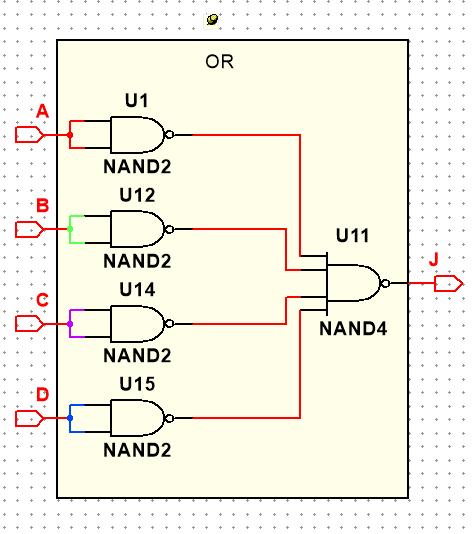
\includegraphics{schemat_J.png}
  \captionof{figure}{Podschemat funkcji logicznej dla członu J} 
\end{figure}


\subsubsection{Transkoder I}
\begin{figure}[H]
 \centering
 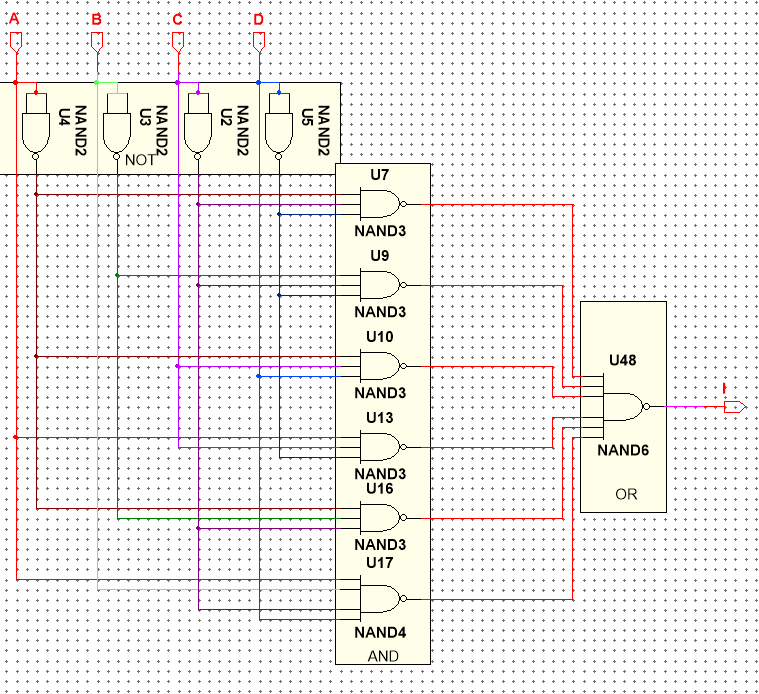
\includegraphics{schemat_I.png}
 \captionof{figure}{Podschemat funkcji logicznej dla członu I} 
\end{figure}


\subsubsection{Transkoder H}
\begin{figure}[H]
 \centering
 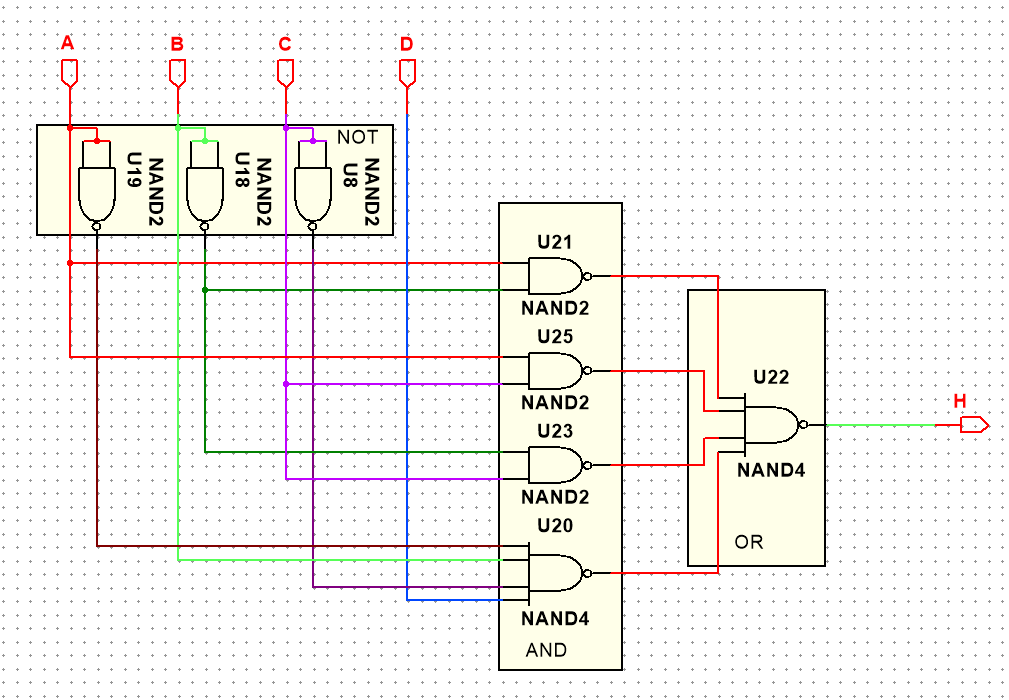
\includegraphics{schemat_H.png}
 \captionof{figure}{Podschemat funkcji logicznej dla członu H} 
\end{figure}

\subsubsection{Transkoder G}
\begin{figure}[H]
 \centering
 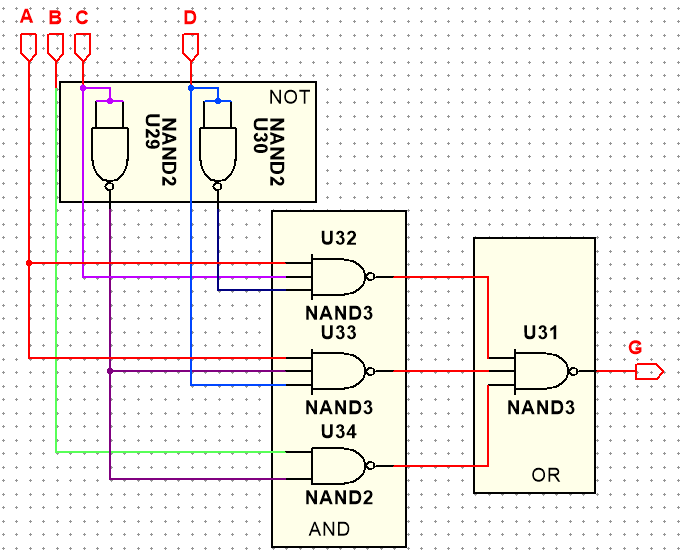
\includegraphics{schemat_G.png}
 \captionof{figure}{Podschemat funkcji logicznej dla członu G} 
\end{figure}

\subsubsection{Transkoder F}
\begin{figure}[H]
 \centering
 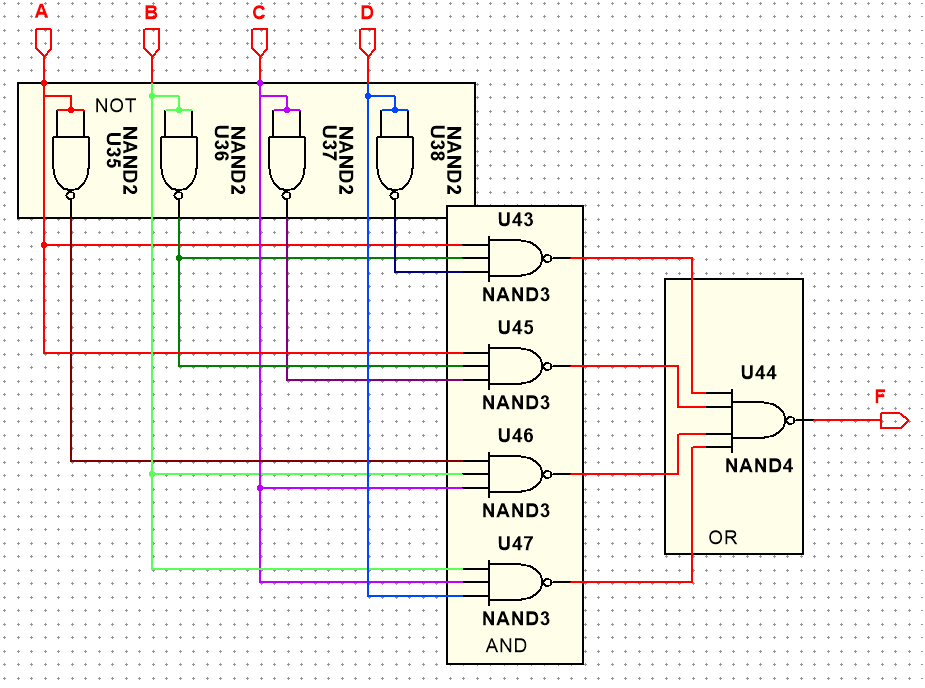
\includegraphics{schemat_F.png}
 \captionof{figure}{Podschemat funkcji logicznej dla członu F} 
\end{figure}

\subsubsection{Transkoder E}
\begin{figure}[H]
 \centering
 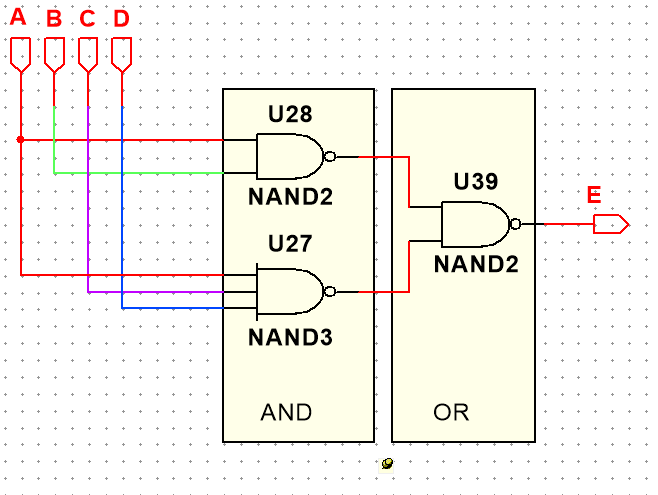
\includegraphics{schemat_E.png}
 \captionof{figure}{Podschemat funkcji logicznej dla członu E} 
\end{figure}
\section{Enkoder BCD}
Aby wyświetlać liczby dwucyfrowe w poprawny sposób zdecydowaliśmy się na zaimplementowanie enkodera BCD (Binary Coded Decimal). Jest to format
w którym liczba dziesiętna jest kodowana cyfra po cyfrze przez 4 bitowe liczby binarne. Pozwala to na łatwe wyświetlanie wielocyfrowych liczb.
W programie Multisim nie udało nam się znaleźć gotowego układu z większą niż 4 bity liczbą wejść, dlatego sami go zaimplementowaliśmy. Jako, że 
nie jest to bezpośredni cel ćwiczenia, nie rozpisywaliśmy ręcznie tablic Karnaugh - dla 6 zmiennych wejściowych jest to bardziej złożona operacja, lecz
skorzystaliśmy z gotowego kalkulatora w internecie (http://www.32x8.com/var6.html), aby wygenerować funkcję logiczną. Tabelę prawd wygenerowaliśmy samemu algorytmicznie, a następnie
zaznaczyliśmy odpowiednie bity w kalkulatorze online w ten sposób otrzymując funkcje logiczne. Użyliśmy go dwukrotnie. Jeden służy do przedstawienia liczb 0-15,
 drugi zaś do przedstawienia kolejnych liczb pierwszych. 
\subsection{Black box}
\begin{figure}[H]
  \centering
  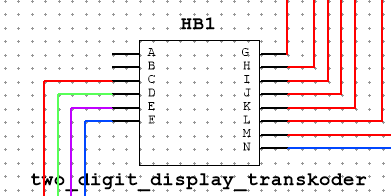
\includegraphics[width=\textwidth]{black_box2.png}
  \captionof{figure}{Czarna skrzynka enkodera BCD dla wejścia} 
\end{figure}
\begin{figure}[H]
  \centering
  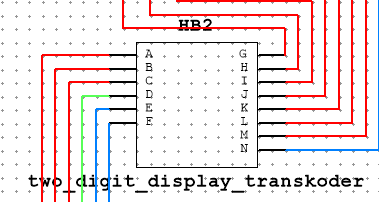
\includegraphics[width=\textwidth]{black_box3.png}
  \captionof{figure}{Czarna skrzynka enkodera BCD dla wyjścia} 
\end{figure}

Wejście do układu stanowią 6 pinów ABCDEF kodujące binarnie wejściową liczbę 0-63. Stan wysoki na pinach
stanowi logiczną jedynkę (1), a stan niski logiczne zero (0).
\begin{center}
  \begin{tabular}{|c|c|c|c|c|c|c|c|}
    \hline Numer bitu & 5 & 4 & 3 & 2 & 1 & 0 \\ 
    \hline Bit & A & B & C & D & E & F  \\
    \hline Mnożnik &$2^5$ &$2^4$ & $2^3$ & $2^2$ & $2^1$ & $2^0$  \\
    \hline
  \end{tabular}
  \captionof{table}{Kodowanie pinów ABCDEF} 
\end{center}

Wyjście układu stanowi 8 pinów GHIJKLMN kodujące odzielnie 2 cyfry składające się na liczbę 2 cyfrową. Tak samo jak na wejściu stan wysoki na pinach
stanowi logiczną jedynkę (1), a stan niski logiczne zero (0). 
\begin{center}
  \begin{tabular}{|c|c|c|c|c|c|c|c|c|}
    \hline Numer bitu & 7 & 6 & 5 & 4 & 3 & 2 & 1 & 0 \\ 
    \hline Bit & G & H & I & J & K & L & M & N \\
    \hline Mnożnik & $2^7$ & $2^6$ & $2^5$ & $2^4$ & $2^3$ & $2^2$ & $2^1$ & $2^0$ \\
    \hline
  \end{tabular}
  \captionof{table}{Kodowanie pinów GHIJKLMN} 
\end{center}

Układ mapuje wejście na wyjście w następujący sposób - zakładając notację binarną zapisanego mapowania.

\begin{center}
  \begin{tabular}{|c|c|c|c|c|c|c|c|c|c|c|c|c|c|c|c|c|}
  \hline Wejście & 0 & 1 & 2 & 3 & 4 & 5 & 6 & 7 & 8 & 9 & 10 & ... & 63 \\
  \hline Oczekiwane wyjście & 0|0 & 0|1 & 0|2 & 0|3 & 0|4 & 0|5 & 0|6 & 0|7 & 0|8 & 0|9 & 1|0 & ... & 6|3 \\
  \hline
  \end{tabular}
  \captionof{table}{Mapowanie wejścia na wyjście} 
  \end{center}

\pagebreak
\subsection{Tabela prawdy}
Poniżej zapisaliśmy tabelę prawd dla projektowanego układu:
\begin{center}
  \begin{tabular}{|c|c|c|c|c|c||c|c|c|c|c|c|c|c|}
  \hline \multicolumn{6}{|c||}{Wejście} & \multicolumn{8}{|c|}{Wyjście} \\
  \hline A & B & C & D & E & F & G   &    H & I & J & K & L & M & N \\
  \hline 0 & 0 & 0 & 0 & 0 & 0 & 0   &  	0 &	0 &	0 &	0 &	0	& 0	& 0 \\
  \hline 0 & 0 & 0 & 0 & 0 & 1 & 0   &  	0 &	0 &	0 &	0 &	0	& 0	& 1 \\
  \hline 0 & 0 & 0 & 0 & 1 & 0 & 0   &  	0 &	0 &	0 &	0 &	0	& 1	& 0 \\
  \hline 0 & 0 & 0 & 0 & 1 & 1 & 0   &  	0 &	0 &	0 &	0 &	0	& 1	& 1 \\
  \hline 0 & 0 & 0 & 1 & 0 & 0 & 0   &  	0 &	0 &	0 &	0 &	1	& 0	& 0 \\
  \hline 0 & 0 & 0 & 1 & 0 & 1 & 0   &  	0 &	0 &	0 &	0 &	1	& 0	& 1 \\
  \hline 0 & 0 & 0 & 1 & 1 & 0 & 0   &  	0 &	0 &	0 &	0 &	1	& 1	& 0 \\
  \hline 0 & 0 & 0 & 1 & 1 & 1 & 0   &  	0 &	0 &	0 &	0 &	1	& 1	& 1 \\
  \hline 0 & 0 & 1 & 0 & 0 & 0 & 0   &  	0 &	0 &	0 &	1 &	0	& 0	& 0 \\
  \hline 0 & 0 & 1 & 0 & 0 & 1 & 0   &  	0 &	0 &	0 &	1 &	0	& 0	& 1 \\
  \hline 0 & 0 & 1 & 0 & 1 & 0 & 0   &  	0 &	0 &	1 &	0 &	0	& 0	& 0 \\
  \hline 0 & 0 & 1 & 0 & 1 & 1 & 0   &  	0 &	0 &	1 &	0 &	0	& 0	& 1 \\
  \hline 0 & 0 & 1 & 1 & 0 & 0 & 0   &  	0 &	0 &	1 &	0 &	0	& 1	& 0 \\
  \hline 0 & 0 & 1 & 1 & 0 & 1 & 0   &  	0 &	0 &	1 &	0 &	0	& 1	& 1 \\
  \hline 0 & 0 & 1 & 1 & 1 & 0 & 0   &  	0 &	0 &	1 &	0 &	1	& 0	& 0 \\
  \hline 0 & 0 & 1 & 1 & 1 & 1 & 0   &  	0 &	0 &	1 &	0 &	1	& 0	& 1 \\
  \hline 0 & 1 & 0 & 0 & 0 & 0 & 0   &  	0 &	0 &	1 &	0 &	1	& 1	& 0 \\
  \hline 0 & 1 & 0 & 0 & 0 & 1 & 0   &  	0 &	0 &	1 &	0 &	1	& 1	& 1 \\
  \hline 0 & 1 & 0 & 0 & 1 & 0 & 0   &  	0 &	0 &	1 &	1 &	0	& 0	& 0 \\
  \hline 0 & 1 & 0 & 0 & 1 & 1 & 0   &  	0 &	0 &	1 &	1 &	0	& 0	& 1 \\
  \hline 0 & 1 & 0 & 1 & 0 & 0 & 0   &  	0 &	1 &	0 &	0 &	0	& 0	& 0 \\
  \hline 0 & 1 & 0 & 1 & 0 & 1 & 0   &  	0 &	1 &	0 &	0 &	0	& 0	& 1 \\
  \hline 0 & 1 & 0 & 1 & 1 & 0 & 0   &  	0 &	1 &	0 &	0 &	0	& 1	& 0 \\
  \hline 0 & 1 & 0 & 1 & 1 & 1 & 0   &  	0 &	1 &	0 &	0 &	0	& 1	& 1 \\
  \hline 0 & 1 & 1 & 0 & 0 & 0 & 0   &  	0 &	1 &	0 &	0 &	1	& 0	& 0 \\
  \hline 0 & 1 & 1 & 0 & 0 & 1 & 0   &  	0 &	1 &	0 &	0 &	1	& 0	& 1 \\
  \hline 0 & 1 & 1 & 0 & 1 & 0 & 0   &  	0 &	1 &	0 &	0 &	1	& 1	& 0 \\
  \hline 0 & 1 & 1 & 0 & 1 & 1 & 0   &  	0 &	1 &	0 &	0 &	1	& 1	& 1 \\
  \hline 0 & 1 & 1 & 1 & 0 & 0 & 0   &  	0 &	1 &	0 &	1 &	0	& 0	& 0 \\
  \hline 0 & 1 & 1 & 1 & 0 & 1 & 0   &  	0 &	1 &	0 &	1 &	0	& 0	& 1 \\
  \hline 0 & 1 & 1 & 1 & 1 & 0 & 0   &  	0 &	1 &	1 &	0 &	0	& 0	& 0 \\
  \hline 0 & 1 & 1 & 1 & 1 & 1 & 0   &  	0 &	1 &	1 &	0 &	0	& 0	& 1 \\
  \hline
  \end{tabular}
\end{center} 
\pagebreak
cd.
\begin{center}
  \begin{tabular}{|c|c|c|c|c|c||c|c|c|c|c|c|c|c|}
  \hline \multicolumn{6}{|c||}{Wejście} & \multicolumn{8}{|c|}{Wyjście} \\
  \hline A & B & C & D & E & F & G   &    H & I & J & K & L & M & N \\
  \hline 1 & 0 & 0 & 0 & 0 & 0 & 0   &  	0 &	1 &	1 &	0 &	0	& 1	& 0 \\
  \hline 1 & 0 & 0 & 0 & 0 & 1 & 0   &  	0 &	1 &	1 &	0 &	0	& 1	& 1 \\
  \hline 1 & 0 & 0 & 0 & 1 & 0 & 0   &  	0 &	1 &	1 &	0 &	1	& 0	& 0 \\
  \hline 1 & 0 & 0 & 0 & 1 & 1 & 0   &  	0 &	1 &	1 &	0 &	1	& 0	& 1 \\
  \hline 1 & 0 & 0 & 1 & 0 & 0 & 0   &  	0 &	1 &	1 &	0 &	1	& 1	& 0 \\
  \hline 1 & 0 & 0 & 1 & 0 & 1 & 0   &  	0 &	1 &	1 &	0 &	1	& 1	& 1 \\
  \hline 1 & 0 & 0 & 1 & 1 & 0 & 0   &  	0 &	1 &	1 &	1 &	0	& 0	& 0 \\
  \hline 1 & 0 & 0 & 1 & 1 & 1 & 0   &  	0 &	1 &	1 &	1 &	0	& 0	& 1 \\
  \hline 1 & 0 & 1 & 0 & 0 & 0 & 0   &  	1 &	0 &	0 &	0 &	0	& 0	& 0 \\
  \hline 1 & 0 & 1 & 0 & 0 & 1 & 0   &  	1 &	0 &	0 &	0 &	0	& 0	& 1 \\
  \hline 1 & 0 & 1 & 0 & 1 & 0 & 0   &  	1 &	0 &	0 &	0 &	0	& 1	& 0 \\
  \hline 1 & 0 & 1 & 0 & 1 & 1 & 0   &  	1 &	0 &	0 &	0 &	0	& 1	& 1 \\
  \hline 1 & 0 & 1 & 1 & 0 & 0 & 0   &  	1 &	0 &	0 &	0 &	1	& 0	& 0 \\
  \hline 1 & 0 & 1 & 1 & 0 & 1 & 0   &  	1 &	0 &	0 &	0 &	1	& 0	& 1 \\
  \hline 1 & 0 & 1 & 1 & 1 & 0 & 0   &  	1 &	0 &	0 &	0 &	1	& 1	& 0 \\
  \hline 1 & 0 & 1 & 1 & 1 & 1 & 0   &  	1 &	0 &	0 &	0 &	1	& 1	& 1 \\
  \hline 1 & 1 & 0 & 0 & 0 & 0 & 0   &  	1 &	0 &	0 &	1 &	0	& 0	& 0 \\
  \hline 1 & 1 & 0 & 0 & 0 & 1 & 0   &  	1 &	0 &	0 &	1 &	0	& 0	& 1 \\
  \hline 1 & 1 & 0 & 0 & 1 & 0 & 0   &  	1 &	0 &	1 &	0 &	0	& 0	& 0 \\
  \hline 1 & 1 & 0 & 0 & 1 & 1 & 0   &  	1 &	0 &	1 &	0 &	0	& 0	& 1 \\
  \hline 1 & 1 & 0 & 1 & 0 & 0 & 0   &  	1 &	0 &	1 &	0 &	0	& 1	& 0 \\
  \hline 1 & 1 & 0 & 1 & 0 & 1 & 0   &  	1 &	0 &	1 &	0 &	0	& 1	& 1 \\
  \hline 1 & 1 & 0 & 1 & 1 & 0 & 0   &  	1 &	0 &	1 &	0 &	1	& 0	& 0 \\
  \hline 1 & 1 & 0 & 1 & 1 & 1 & 0   &  	1 &	0 &	1 &	0 &	1	& 0	& 1 \\
  \hline 1 & 1 & 1 & 0 & 0 & 0 & 0   &  	1 &	0 &	1 &	0 &	1	& 1	& 0 \\
  \hline 1 & 1 & 1 & 0 & 0 & 1 & 0   &  	1 &	0 &	1 &	0 &	1	& 1	& 1 \\
  \hline 1 & 1 & 1 & 0 & 1 & 0 & 0   &  	1 &	0 &	1 &	1 &	0	& 0	& 0 \\
  \hline 1 & 1 & 1 & 0 & 1 & 1 & 0   &  	1 &	0 &	1 &	1 &	0	& 0	& 1 \\
  \hline 1 & 1 & 1 & 1 & 0 & 0 & 0   &  	1 &	1 &	0 &	0 &	0	& 0	& 0 \\
  \hline 1 & 1 & 1 & 1 & 0 & 1 & 0   &  	1 &	1 &	0 &	0 &	0	& 0	& 1 \\
  \hline 1 & 1 & 1 & 1 & 1 & 0 & 0   &  	1 &	1 &	0 &	0 &	0	& 1	& 0 \\
  \hline 1 & 1 & 1 & 1 & 1 & 1 & 0   &  	1 &	1 &	0 &	0 &	0	& 1	& 1 \\
  \hline 
  \end{tabular}
  \captionof{table}{Tabela prawdy dla układu} 
\end{center} 

% y = A'B'C'E + A'C'DE + AB'C'E' +
%  + AC'DE' + AB'CE + ACDE + A'B'CDE' + A'BC'D'E' + A'BCD'E + ABCD'E'

\subsection{Funkcje logiczne}
\subsubsection{Funkcja M}
\begin{center}
  $f_{(1)} = 
    {\overline{ABC}E} +
    {\overline{AC}DE} + 
    {A\overline{BCE}} +
    {A\overline{C}D\overline{E}} +
    {A\overline{B}CE} +
    {ACDE}+
    {\overline{AB}CD\overline{E}} +
    {\overline{A}B\overline{CDE}} +
    {\overline{A}BC\overline{D}E} +
    {ABC\overline{DE}} $
\end{center}

% y = A'B'C'D + B'CDE + A'BD'E' + A'BCD' + BCD'E' + AB'DE' + AB'C'D'E + ABC'DE

\subsubsection{Funkcja L}
\begin{center}
  $f_{(1)} = 
  {\overline{ABC}D} + 
  {\overline{B}CDE} +
  {\overline{A}B\overline{DE}} +
  {\overline{A}BC\overline{D}} +
  {BC\overline{DE}} +
  {A\overline{B}D\overline{E}} +
  {A\overline{BCD}E} +
  {AB\overline{C}DE} $
\end{center}

% y = A'B'CD'E' + A'BC'D'E + A'BCDE' + AB'C'DE + ABC'D'E' + ABCD'E

\subsubsection{Funkcja K}
\begin{center}
  $f_{(1)} = 
  {\overline{AB}C\overline{DE}} +
  {\overline{A}B\overline{CD}E} +
  {\overline{A}BCD\overline{E}} +
  {A\overline{BC}DE} +
  {AB\overline{CDE}} +
  {ABC\overline{D}E} $
\end{center}

% y = AB'C' + AC'E + AC'D + A'B'CE + A'B'CD + A'CDE + A'BC'D' + ABCD'

\subsubsection{Funkcja J}
\begin{center}
  $f_{(1)} = 
  {A\overline{BC}} +
  {A\overline{C}E} +
  {A\overline{C}D} +
  {\overline{AB}CE} +
  {\overline{AB}CD} +
  {\overline{A}CDE} +
  {\overline{A}B\overline{CD}} +
  {ABC\overline{D}} $
\end{center}

% y = A'BD + A'BC + BCD + AB'C'

\subsubsection{Funkcja I}
\begin{center}
  $f_{(1)} = 
  {\overline{A}BD} +
  {\overline{A}BC} +
  {BCD} +
  {A\overline{BC}} $
\end{center}

% y = AC + AB

\subsubsection{Funkcja H}
\begin{center}
  $f_{(1)} = {AB} + {AB} $
\end{center}

\subsection{Implementacja}
Tak jak poprzednio, otrzymane funkcje logiczne zostały w naszym układzie zaimplementowane wyłącznie przy użyciu bramek NAND.
  Tutaj również wykorzystaliśmy schematy hierarchiczne, zachowując, ten sam co wcześniej, podział na czerną skrzynkę, główny podschemat i transkodery dla poszczególnych bitów.
\begin{figure}[H]
  \centering
  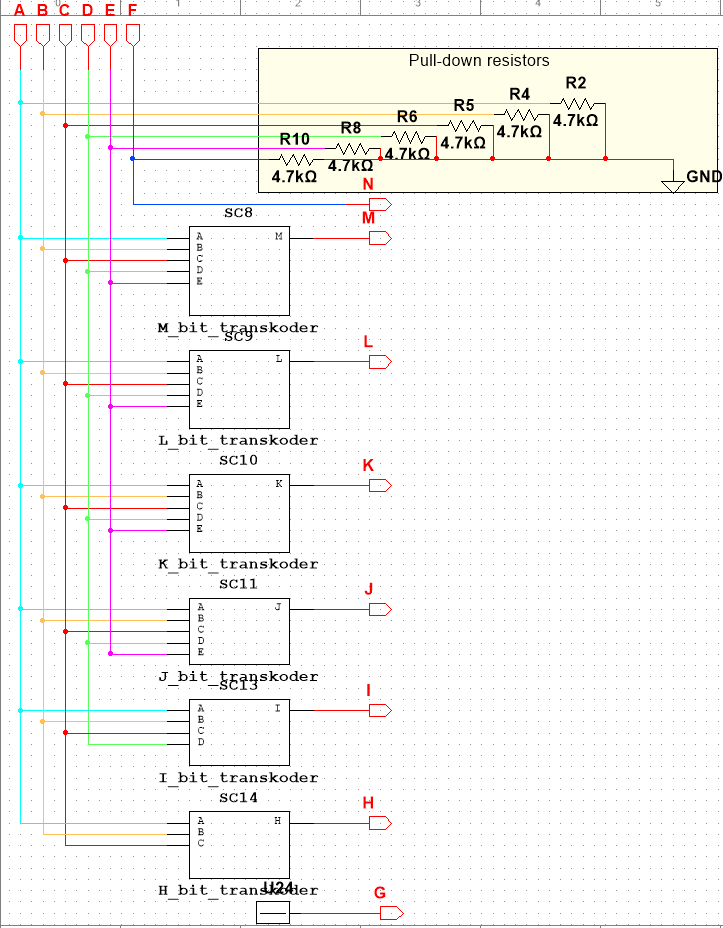
\includegraphics[width=\textwidth]{enkoder_bcd.png}
  \label{Podschemat najwyższego rzędu, gromadzący w sobie podschematy właściwych funkcji logicznych}
  \captionof{figure}{Podschemat najwyższego rzędu, gromadzący w sobie podschematy właściwych funkcji logicznych} 
\end{figure}


\subsubsection{Enkoder M}
 \begin{figure}[H]
  \centering
  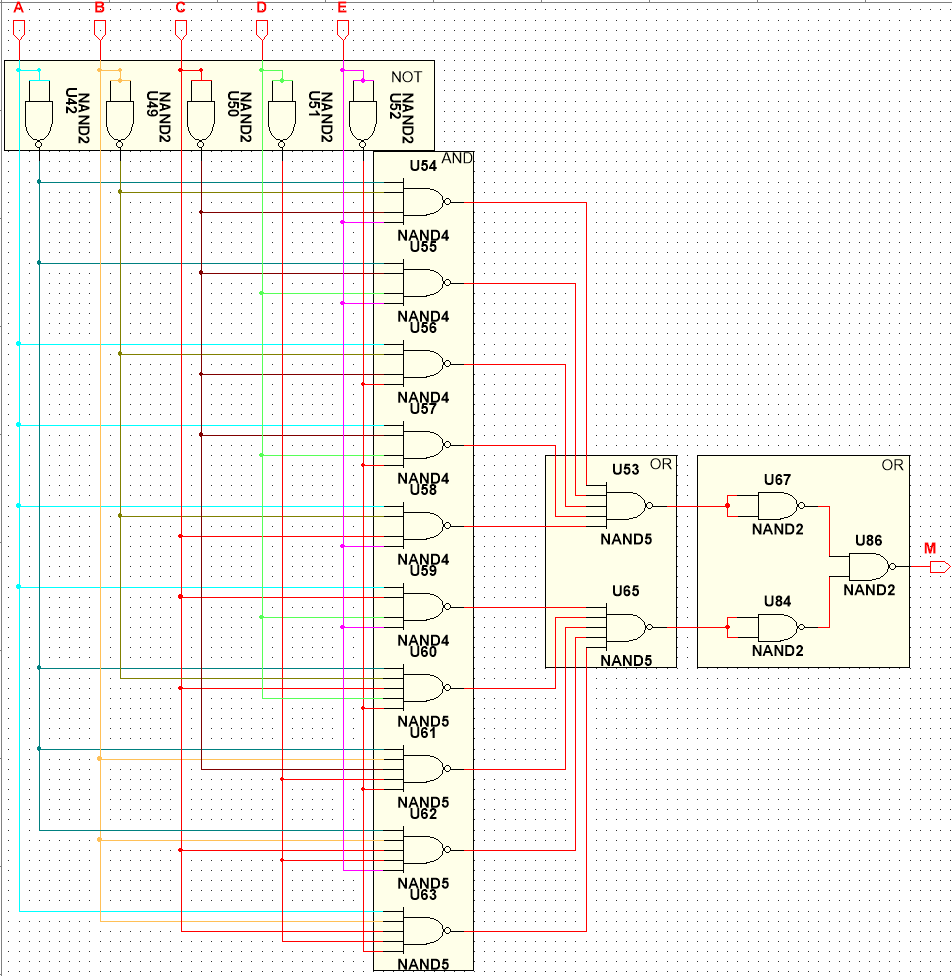
\includegraphics[width=\linewidth]{enkoder_bcd_M.png}
  \captionof{figure}{Podschemat funkcji logicznej dla członu M} 
\end{figure}


\subsubsection{Enkoder L}
\begin{figure}[H]
 \centering
 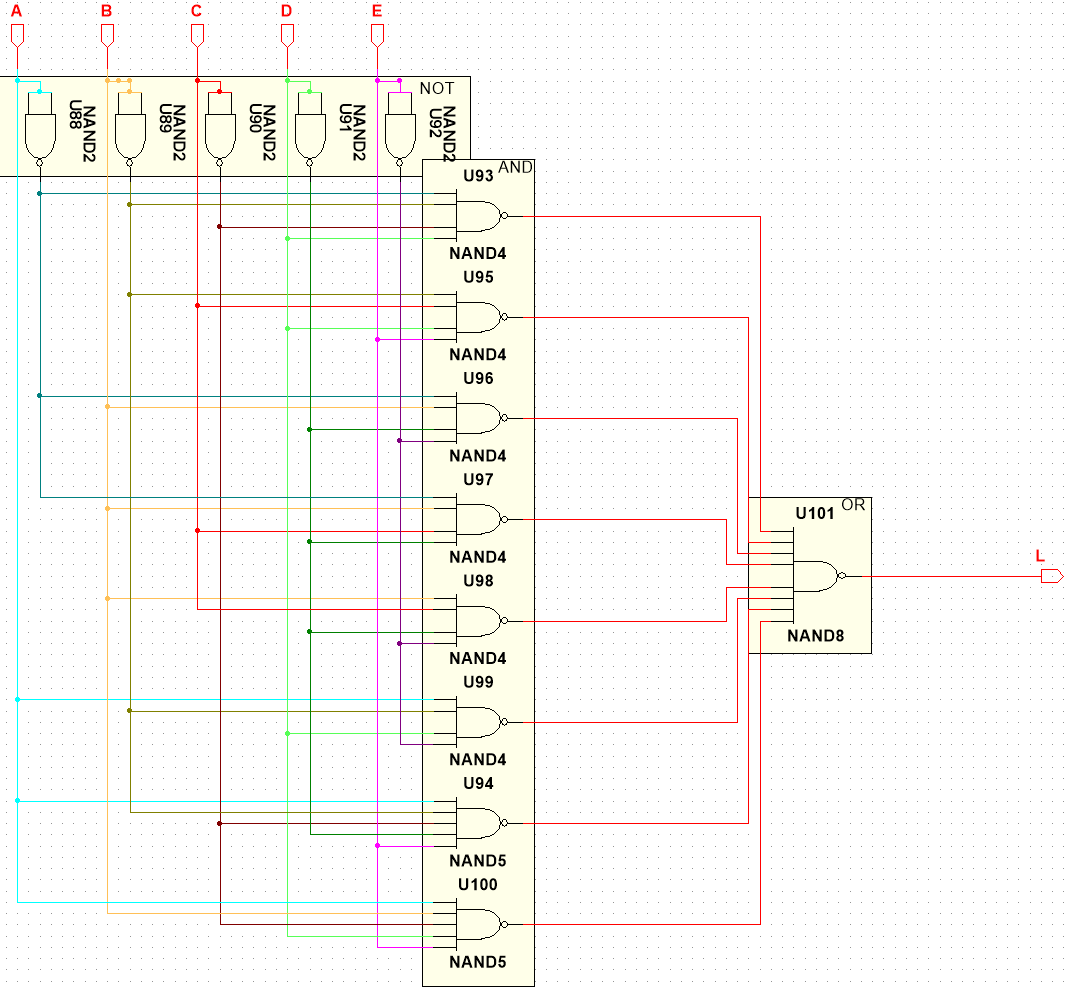
\includegraphics[width=\linewidth]{enkoder_bcd_L.png}
 \captionof{figure}{Podschemat funkcji logicznej dla członu L} 
\end{figure}


\subsubsection{Enkoder K}
\begin{figure}[H]
 \centering
 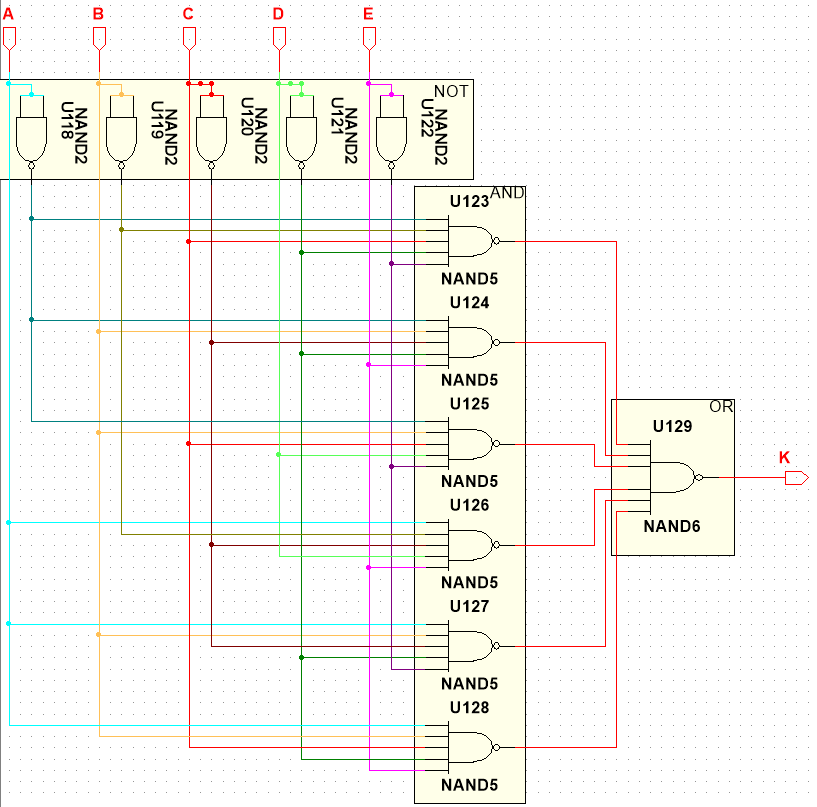
\includegraphics{enkoder_bcd_K.png}
 \captionof{figure}{Podschemat funkcji logicznej dla członu K} 
\end{figure}

\subsubsection{Enkoder J}
\begin{figure}[H]
 \centering
 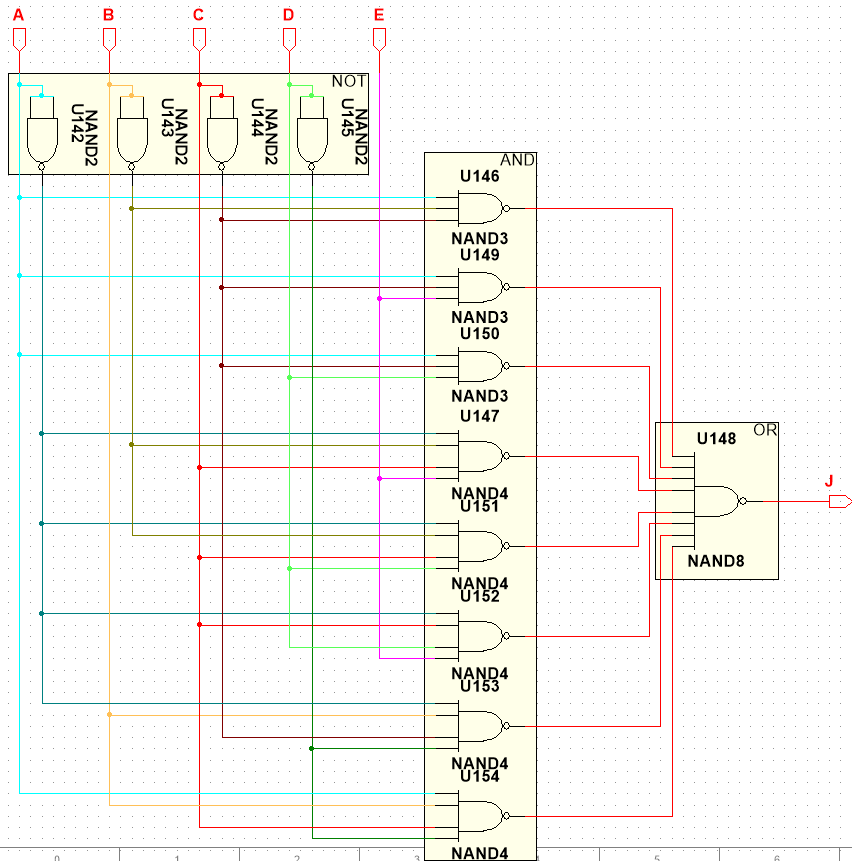
\includegraphics{enkoder_bcd_J.png}
 \captionof{figure}{Podschemat funkcji logicznej dla członu J} 
\end{figure}

\subsubsection{Enkoder I}
\begin{figure}[H]
 \centering
 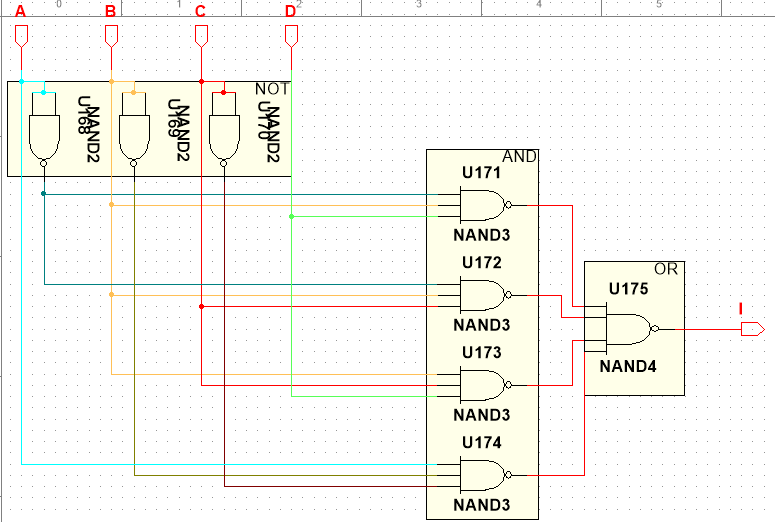
\includegraphics{enkoder_bcd_I.png}
 \captionof{figure}{Podschemat funkcji logicznej dla członu I} 
\end{figure}

\subsubsection{Enkoder H}
\begin{figure}[H]
 \centering
 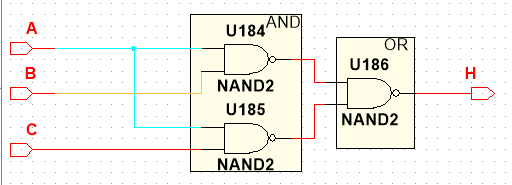
\includegraphics{enkoder_bcd_H.png}
 \captionof{figure}{Podschemat funkcji logicznej dla członu H} 
\end{figure}

\section{Układ testowy}
Aby przetestować projektowany element zestawiliśmy układ zawierający:
\begin{itemize}
  \item Word Generator - generuje 4 bity wejściowe dla naszego układu, oraz 6 bitów oczekiwanego wyjścia - zakodowane liczby pierwsze
  \item Comparator - porównuje wyjście układu z zakodowanym wyjściem z generatora sygnałów
  \item Logic Analyzer - pozwala na wyświetlenie przebiegów wejścia i wyjścia układu, aby sprawdzić poprawność jego działania
  \item Wyświetlacze HEX - wyświetlacze 7 segmentowe z enkoderem pozwalające wyświetlić liczby 0-15 jako cyfry szesnastkowe
  \item Prime transkoder - nasz zaprojektowany układ transkodujący liczby 0-15 na liczby pierwsze
  \item two digit display transkoder - nasz autorski enkoder BCD, pozwalający lepiej zwizualizować działanie naszego układu
\end{itemize}

\begin{figure}[H]
  \centering
  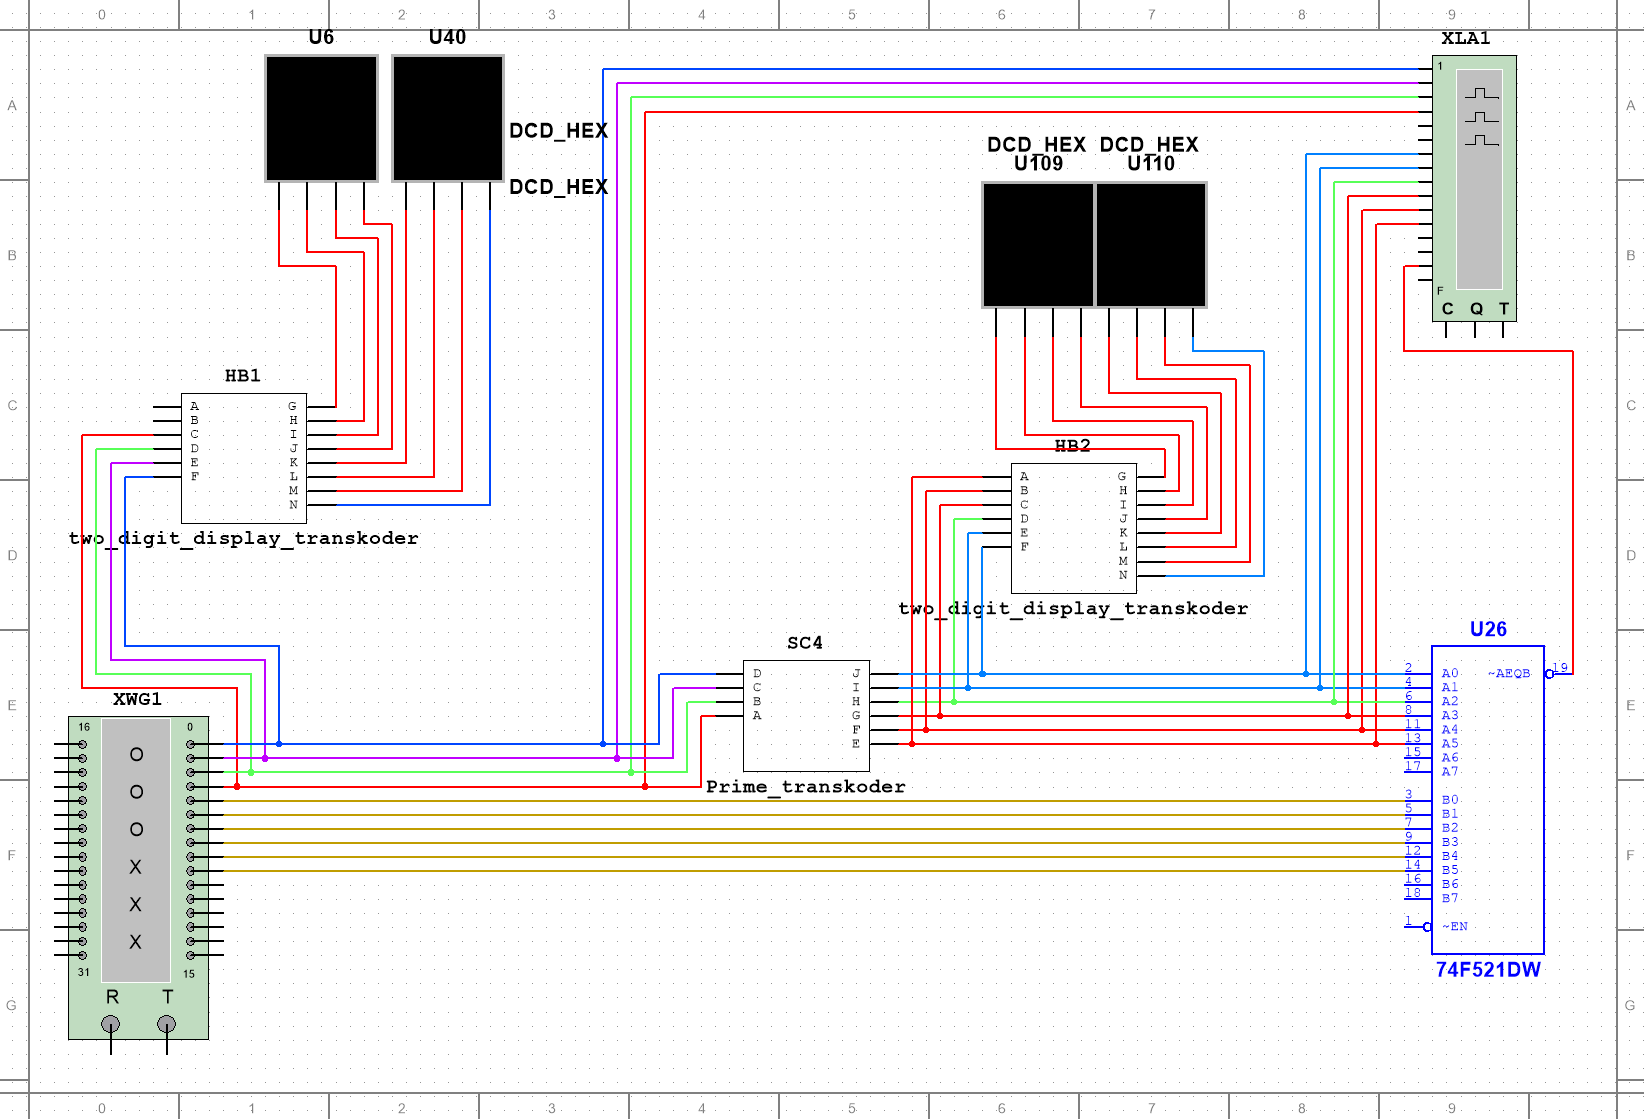
\includegraphics[width=\linewidth]{schemat.png}
  \captionof{figure}{Schemat całego układu} 
 \end{figure}

\subsection{Analiza przebiegu}
\begin{itemize}
  \item{Word Generator}
   \subitem{Generuje 4 bity wejściowe dla układu, które są następnie przesyłane do Prime Transkodera oraz do Two Digit Display Transkodera.}
   \subitem{Generuje 6 bitów oczekiwanego wyjścia, które są zakodowanymi liczbami pierwszymi. Te bity są porównywane przez Comparator z wyjściem Prime Transkodera.}
  \item{Prime Transkoder}
   \subitem{Otrzymuje 4 bity wejściowe od Word Generator.}
   \subitem{Transkoduje otrzymane bity wejściowe na liczby pierwsze zgodnie z opisaną tabelą.}
   \subitem{Wygenerowane liczby pierwsze są przekazywane do Comparatora w celu porównania z oczekiwanym wyjściem.}
  \item{Comperator}
   \subitem{Porównuje wyjście z Prime Transkodera (liczby pierwsze) z zakodowanymi liczbami pierwszymi wygenerowanymi przez Word Generator.}
   \subitem{Jeśli wyjście układu jest zgodne z oczekiwanym wyjściem, generuje sygnał informujący o poprawności działania układu.}

  \item{Two Digit Display Transkoder}
    \subitem{Pierwszy z nich otrzymuje od Word Generatora 4 bity wejściowe i transkoduje je zgodnie z opisaną tabelą, a następnie przekazuje do wyświetlaczy HEX}
    \subitem{Drugi z nich otrzymuje od Prime Transkodera 6 bitów wejściowych i transkoduje je zgodnie z opisaną tabelą, a następnie przekazuje do wyświetlaczy HEX}

  \item{Wyświetlacze HEX}
   \subitem{Pomagają w lepszym zobrazowaniu działania układu poprzez wizualizację zadanych liczb.}
   \pagebreak
  \item{Logic Analyzer}
  \begin{figure}[H]
    \centering
    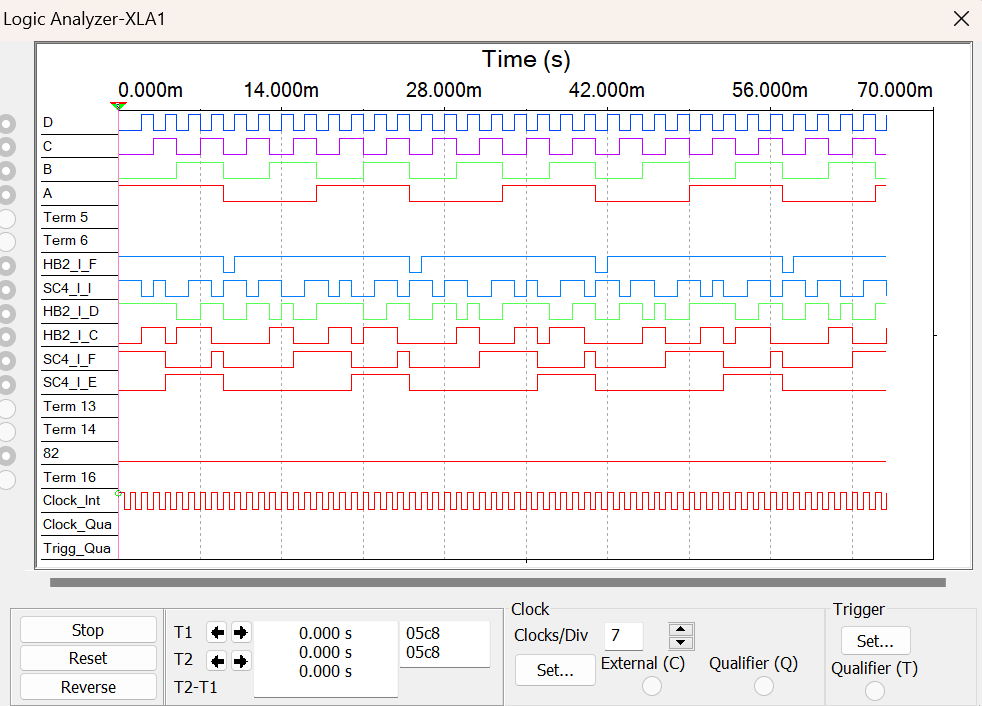
\includegraphics[width=\linewidth]{logicAnalyzer.png}
    \captionof{figure}{Zrzut ekranu z analizatora logicznego w trakcie działania układu} 
  \end{figure}
\end{itemize}


\section{Zastosowania}
Poniżej wymieniamy przykładowe zastosowania zaprojektowanego układu:
\begin{itemize}
  \item Transkoder generujący liczby pierwsze na podstawie prostej liczby może być zastosowany w urządzeniach 
      szyfrujących. Dużo łatwiej jest wygenerować (pseudo)-losową liczbę z przedziału 0-15 i ją przekształcić na
      liczbę pierwszą za pomocą takiego transkodera niż wybierać losową liczbę pierwszą. Wiele algorytmów szyfrujących
      czy funkcji hashujących bazuje na liczbach pierwszych więc taki układ miałby tam zastosowanie.
  \item Innym zastosowaniem układów z rodziny transkoderów - lecz nie koniecznie tego konkretnego - może być 
      przekształcenie kodu jakiegoś błędu reprezentowanego w systemie przez liczby 0-15 na jakiś inny kod błędu, 
      który np. nadaje się do wyświetlenia użytkownikowi - bo mówi coś więcej o istocie problemu.
\end{itemize}
\end{document}


